\documentclass[11pt]{article}

\usepackage[english]{babel}
\usepackage[T1]{fontenc}
\usepackage[utf8x]{inputenc}

\usepackage{appendix}
\usepackage{amsmath}
\usepackage{cprotect}
\usepackage{listings}
\usepackage{float}
\usepackage[margin=2cm]{geometry}
\usepackage{graphicx}
\usepackage{underscore}

\lstset{
    tabsize=3,
    breakatwhitespace=true,
    breaklines=true,
    frame=simple
}

\title{Lab2 - FPGA Placer}
\author{Matthew Walker - 999540475 - walker82}
\date{\today}

%TODO HPBBWL for each circuit
%TODO compare snapped vs not snapped
%TODO program flow

\begin{document}

\maketitle

\section{Results}
\subsection{Numbers}
\begin{table}[ht]
\centering\begin{tabular}{ c *3r}
\hline\hline
Circuit & As Solved & After Final Legalization & Increase \\
\hline
cct1 & 133.15  & 146   & 9.6\% \\
cct2 & 1376.63 & 1443  & 4.8\% \\
cct3 & 9651.9  & 10414 & 7.8\% \\
cct4 & 30959.2 & 32610 & 5.3\% \\
\hline\hline
\end{tabular}
\caption{Half-perimeter-bounding-box wire lengths. \label{tab:hpbbwl}}
\end{table}

\subsection{Discussion}
The observed 5-10\% increase in HPBBWL is likely due to localized insufficient spreading, requiring blocks that must be placed in non-ideal locations. Most of the increase is probably due to: sets of blocks whose solution location is closer together than the block spacing; and the fact that the spreading never quite manages to stretch the circuit out to fill the entire device completely before the stopping condition is met, resulting in the entire circuit being stretched out somewhat more. Also, for example, in cct3, one block must be moved all the way to the opposite side of the device, as there are no empty local slots. To deal with that situation, something more sophisticated, such as Simulated Annealing, could reduce the impact.

\section{Approach}
\subsection{Overview}
The approach is iterative. Each iteration divides up the board one level deeper, with a limit. Weights to anchors are decayed exponentially. Once the limit has been reached, no new weights are added: instead, the weights between the last set of anchors and the movable blocks is increased (section \ref{sec:spreading}). The stopping condition is to examine the fraction of blocks that are assigned to the same slot after a snapping (section \ref{sec:snapping}) is computed. If this number from the \emph{previous} iteration is below 20\%, and it increased \emph{this} iteration, then the solution from the previous iteration is accepted. This accepted solution is then run through a more strict legalizer (section \ref{sec:legalizing}) that always produces a snapping with no overlaps.

\subsection{Spreading}\label{sec:spreading}
The method suggested in the handout is used. First the centroid of the to-be-placed blocks is found, then the centroid of each quarter is found, recursively, with the depth limited to the iteration number (initially 0, so no spreading) and to so that the total number of anchors is not more than 8 times the number of blocks. It was found that increasing the density of anchor further did not result in better results, just slower solves. Also, the maximum number of anchors should be at leas the the number of blocks, as using fewer resulted in clumps of blocks, and worse solutions.

Anchor weights are determined by the following formula:
\[10 \cdot 1.1^{3\cdot\text{anchor_gen}} \cdot 2^{\text{anchor_gen } - \text{ iteration_number}}\]
where anchor_gen is the iteration number where the anchors were created, with anchors persisting across iterations. The second exponential implements decaying weights.

\subsection{Snapping}\label{sec:snapping}
The snapping algorithm is as follows:
\begin{enumerate}
\item Slots used by fixed blocks are reserved.
\item The closest block to each slot is placed there.
\item Blocks are sorted according to increasing distance from the centre of the device
\item The unplaced blocks are visited in the sorted order, and the adjacent slots are explored. The one that is both free and closest to the centre of the device is placed chosen for that block. \label{enum:explore-step}
\item Any remaining blocks are simply placed at their ideal location
\end{enumerate}

\subsubsection{Legalization}\label{sec:legalization}
In order to not allow any overlaps, step \ref{enum:explore-step} is repeated until all blocks are placed, but with a distance from the ideal slot one greater each time. 

\section{Software Flow \& Organization}\label{sec:prog-flow}
The relevant files for the this report are \texttt{src/anaplace_main.cpp}, \texttt{flows/placement_flows.cpp}, \texttt{src/ algo/analytic_placement.hpp} and \texttt{src/util/umfpack_interface.cpp}.

\texttt{main} (in \texttt{anaplace_main}) the command line arguments, and then calls \texttt{program_main}, which calls the parser for the input circuit, and then calls \texttt{flows::placement::clique_and_spread} (in \texttt{placement_flows.cpp}. \texttt{clique_and_spread} calls \texttt{flows::placement::CliqueAndSpreadFlow::flow_main} (same file) that contains the main iterative loop. \texttt{CliqueAndSpreadFlow::flow_main} calls \texttt{flows::placement:: SimpleCliqueSolve::flow_main} for finding an exact solution (this calls \texttt{apl::exact_solution} (in \texttt{analytic _placement.hpp}), and \texttt{flows::placement::LegalizationFlow::flow_main} for legalization.

\clearpage
\appendix
\section*{Appendix}

\section{Result Plots}\label{app:result-plots}
\begin{figure}[H]
\centering
\includegraphics[clip, viewport=213 280 443 510, width=7cm]{assets/lab2/cct1-legalized.ps}
\cprotect\caption{\small\verb|anaplace --circuit data/anaplace/cct1.txt --graphics|}
\end{figure}

\begin{figure}[H]
\centering
\includegraphics[clip, viewport=176 247 468 539, width=11cm]{assets/lab2/cct2-legalized.ps}
\cprotect\caption{\small\verb|anaplace --circuit data/anaplace/cct2.txt --graphics|}
\end{figure}

\begin{figure}[H]
\centering
\includegraphics[clip, viewport=171 244 480 548, width=\linewidth]{assets/lab2/cct3-legalized.ps}
\cprotect\caption{\small\verb|anaplace --circuit data/anaplace/cct3.txt --graphics|}
\end{figure}
\begin{figure}[H]
\centering
\includegraphics[clip, viewport=196 269 454 523, width=\linewidth]{assets/lab2/cct4-legalized.ps}
\cprotect\caption{\small\verb|anaplace --circuit data/anaplace/cct4.txt --graphics|}
\end{figure}

\end{document}
